% Pass extraction: coarse bracketing, bisection, golden-section. Illustrative curve.
% Built by experiments/diagrams/build_diagrams.py.
\documentclass[border=4pt]{standalone}
\usepackage{tikz}
\usetikzlibrary{arrows.meta, calc}
\definecolor{orbit}{HTML}{0072B2}
\definecolor{plan}{HTML}{E69F00}
\definecolor{outc}{HTML}{D55E00}
\definecolor{src}{HTML}{666666}
\begin{document}
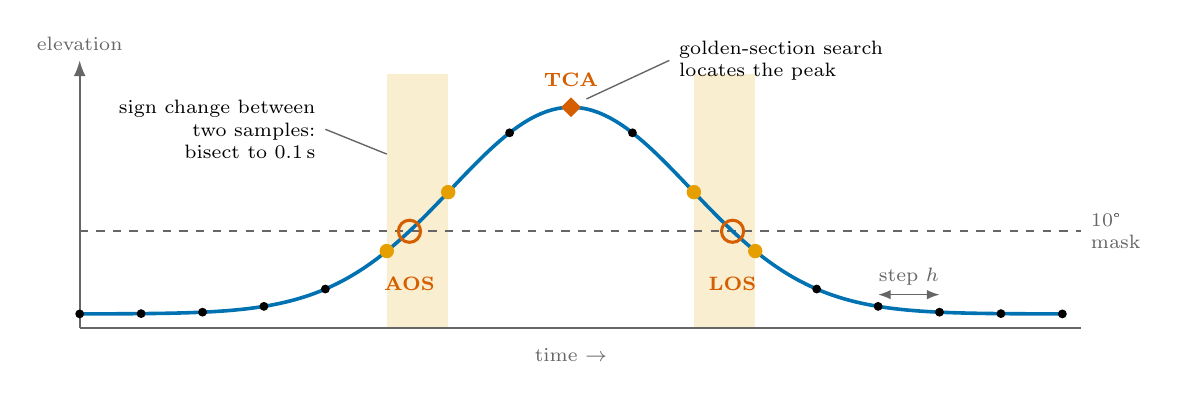
\begin{tikzpicture}[x=0.78cm, y=0.7cm, font=\footnotesize,
  every node/.append style={execute at begin node={\hyphenpenalty=10000}}]
% elevation e(x) = -20 + 75 exp(-((x-8)/2.75)^2) degrees, drawn at e/20 units
\def\elev#1{(-20 + 75*exp(-((#1-8)/2.75)^2))/20}
% brackets that contain the crossings (shaded first, so they sit behind)
\fill[plan!18] (5,-1.25) rectangle (6,3.35);
\fill[plan!18] (10,-1.25) rectangle (11,3.35);
% axes and mask
\draw[src, line width=0.6pt] (0,-1.25) -- (16.3,-1.25);
\draw[src, -{Latex[length=2mm]}, line width=0.6pt] (0,-1.25) -- (0,3.6)
      node[above, font=\scriptsize, text=src] {elevation};
\draw[src, dashed, line width=0.7pt] (0,0.5) -- (16.3,0.5)
      node[right, font=\scriptsize, text=src, align=left] {10\textdegree\\mask};
\node[font=\scriptsize, text=src] at (8,-1.75) {time $\rightarrow$};
% the elevation curve
\draw[orbit, line width=1.3pt, smooth, samples=120, domain=0:16]
     plot (\x, {\elev{\x}});
% coarse samples every step h
\foreach \t in {0,...,16} {
  \pgfmathsetmacro{\e}{\elev{\t}}
  \fill[black] (\t,\e) circle (1.6pt);
}
% bracket samples (sign change of elevation - mask)
\foreach \t in {5,6,10,11} {
  \pgfmathsetmacro{\e}{\elev{\t}}
  \fill[plan] (\t,\e) circle (2.6pt);
}
% AOS, LOS found by bisection
\foreach \t/\lab in {5.37/AOS, 10.63/LOS} {
  \draw[outc, line width=1.1pt] (\t,0.5) circle (4pt);
  \node[text=outc, font=\scriptsize\bfseries, below] at (\t,-0.15) {\lab};
}
% TCA by golden-section search
\fill[outc] (8,3.75-1) ++(0,0.18) -- ++(0.16,-0.18) -- ++(-0.16,-0.18) -- ++(-0.16,0.18) -- cycle;
\node[text=outc, font=\scriptsize\bfseries, above] at (8,2.95) {TCA};
% annotations
\draw[src, line width=0.5pt] (5,1.9) -- (4.0,2.35)
      node[left, font=\scriptsize, align=right, text=black]
      {sign change between\\two samples:\\bisect to 0.1\,s};
\draw[src, line width=0.5pt] (8.25,2.9) -- (9.6,3.6)
      node[right, font=\scriptsize, align=left, text=black]
      {golden-section search\\locates the peak};
% step h
\draw[src, {Latex[length=1.6mm]}-{Latex[length=1.6mm]}, line width=0.5pt] (13,-0.65) -- (14,-0.65);
\node[font=\scriptsize, text=src, above] at (13.5,-0.65) {step $h$};
\end{tikzpicture}
\end{document}
